\documentclass[a4paper,12pt]{article}
\usepackage[left=2.5cm, right=2.5cm, top=2.5cm, bottom=2.5cm]{geometry}
\usepackage[backend=biber]{biblatex}
\addbibresource{../bibliography.bib}
\usepackage{minted}
\setminted{frame=lines, fontsize=\small}
\usepackage{graphicx}
\usepackage{hyperref}
\hypersetup{
    colorlinks=true,
    linkcolor=black,
    filecolor=black,
    urlcolor=black,
    citecolor=black
}

\title{Literature summaries}
\author{Adrià Casanova Lloveras}

\begin{document}

\maketitle

\tableofcontents
\pagebreak

\section{Rdimtools: An R Package for Dimension Reduction
and Intrinsic Dimension Estimation \texorpdfstring{\cite{Rdimtools}}{}}
\label{sec:rdimtools}


\subsection{Abstract}

Discovering patterns of the complex high-dimensional data is one of the fundamental pillars of modern data science. Dimension reduction and intrinsic dimension estimation are two thematic programs that facilitate geometric characterization of the data. We present Rdimtools, an R package that supports 143 dimension reduction and manifold learning methods and 17 dimension estimation algorithms whose unprecedented extent makes multifaceted scrutiny of the data in one place easier. Rdimtools is distributed under the MIT license and is accessible from CRAN, GitHub, and its package website, all of which deliver instruction for installation, self-contained examples, and API documentation.

\subsection{Key Points}

\begin{itemize}
    \item \textbf{R package}: that supports 143 dimension reduction and manifold learning methods and 17 dimension estimation algorithms.
    \item \textbf{Other libraries}: drtoolbox in MATLAB, scikit-learn in Python, a C++ template library tapkee with a known basis of popularity. In R, packages
    dimRed, dyndimred, intrinsicDimension.
    \item \textbf{Implementation}: mixture of R and C++ that are integrated by Rcpp. For numerical operations, RcppArmadillo is heavily used to take advantage of Armadillo C++ linear algebra library.
    \item  \textbf{3 families of functions}: do.\{algorithm\}, est.\{algorithm\},
    and aux.\{algorithm\} for DR, IDE, and auxiliary functions.
    \item Downloaded 1013 times per month on average from CRAN.
    \item \textbf{Future plan}: support for out-of-memory execution in response to the increased needs for big data analysis.
\end{itemize}

\subsection{Example R Code}

\begin{minted}{r}
    # Documentation example:
    # do.idmap (Interactive Document Map)

    library(Rdimtools)

    ## load iris data
    data(iris)
    set.seed(100)
    subid = sample(1:150,50)
    X = as.matrix(iris[subid,1:4])
    lab = as.factor(iris[subid,5])
    ## let's compare with other methods
    out1 <- do.pca(X, ndim=2)
    out2 <- do.lda(X, ndim=2, label=lab)
    out3 <- do.idmap(X, ndim=2, engine="NNP")
    ## visualize
    opar <- par(no.readonly=TRUE)
    par(mfrow=c(1,3))
    plot(out1$Y, pch=19, col=lab, main="PCA")
    plot(out2$Y, pch=19, col=lab, main="LDA")
    plot(out3$Y, pch=19, col=lab, main="IDMAP")
    par(opar)
\end{minted}

\begin{figure}[h]
    \centering
    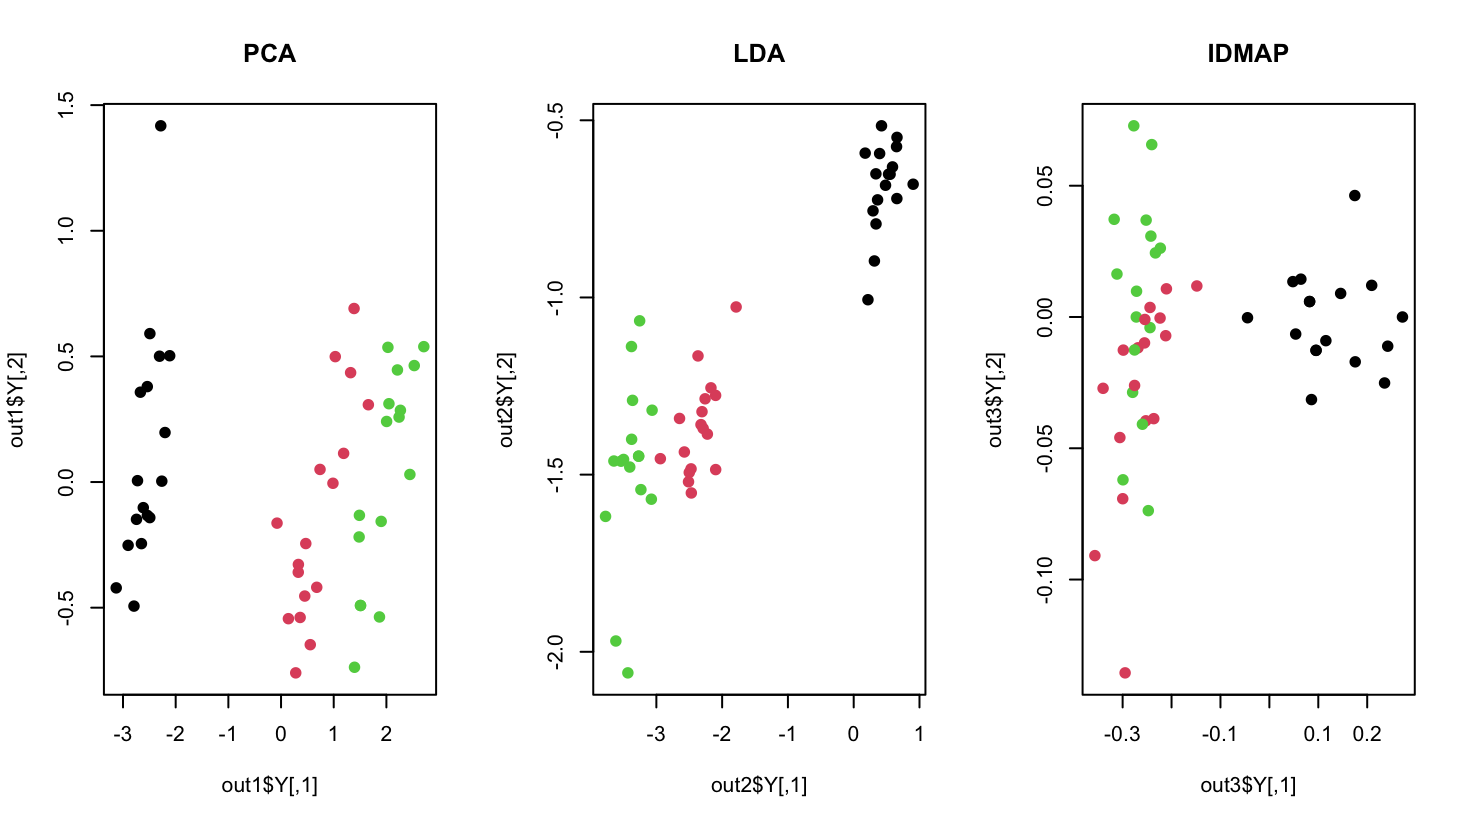
\includegraphics[width=0.8\textwidth]{../../code/Rdimtools_test.png}
    \caption{Rdimtools test output.}
    \label{fig:rdimtools_test}
\end{figure}


\pagebreak
\printbibliography

\end{document}